\chapter{Experiment}
\todo{ne tolle Einleitung schreiben}

\section{Setup A: Estimation of the quadrature point of the MZI modulator}
To calculate the quadrature point of the used MZI modulator the setup shown in figure \ref{fig:A_setup}\footnote[3]{Luca Alloatti, Materials for the preparation of OKT lab 8} was used. A laser source with an output wavelength of 1550~nm and an output power of 0~dBm was connected to an MZI modulator. The output of the MZI modulator was connected to a power meter. The modulator was biased over a variable DC voltage.

The DC voltage was swept from -4.8~V to 5.1~V in steps of 0.3~V. At every point the output power of the MZM was measured.

\begin{figure}%
\centering
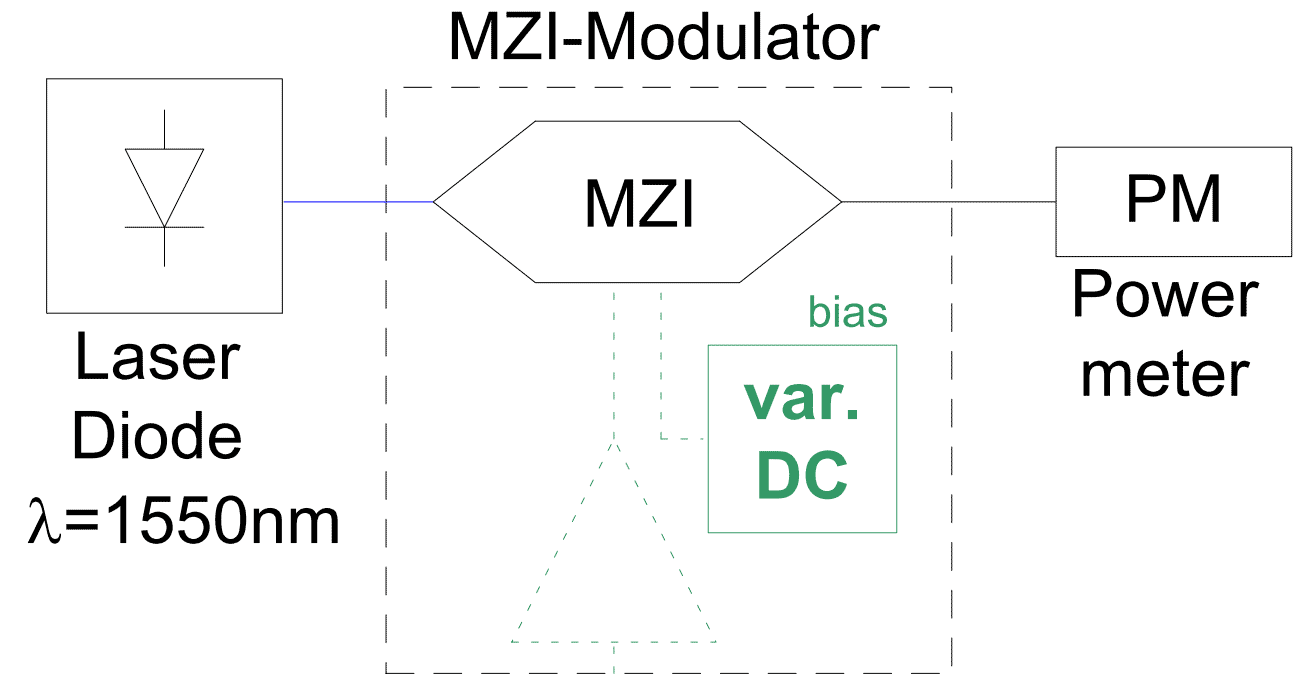
\includegraphics[width=.5\columnwidth]{Grafiken/SetupA.png}%
\caption{Setup A}%
\label{fig:A_setup}%
\end{figure}

\begin{figure}%
\centering
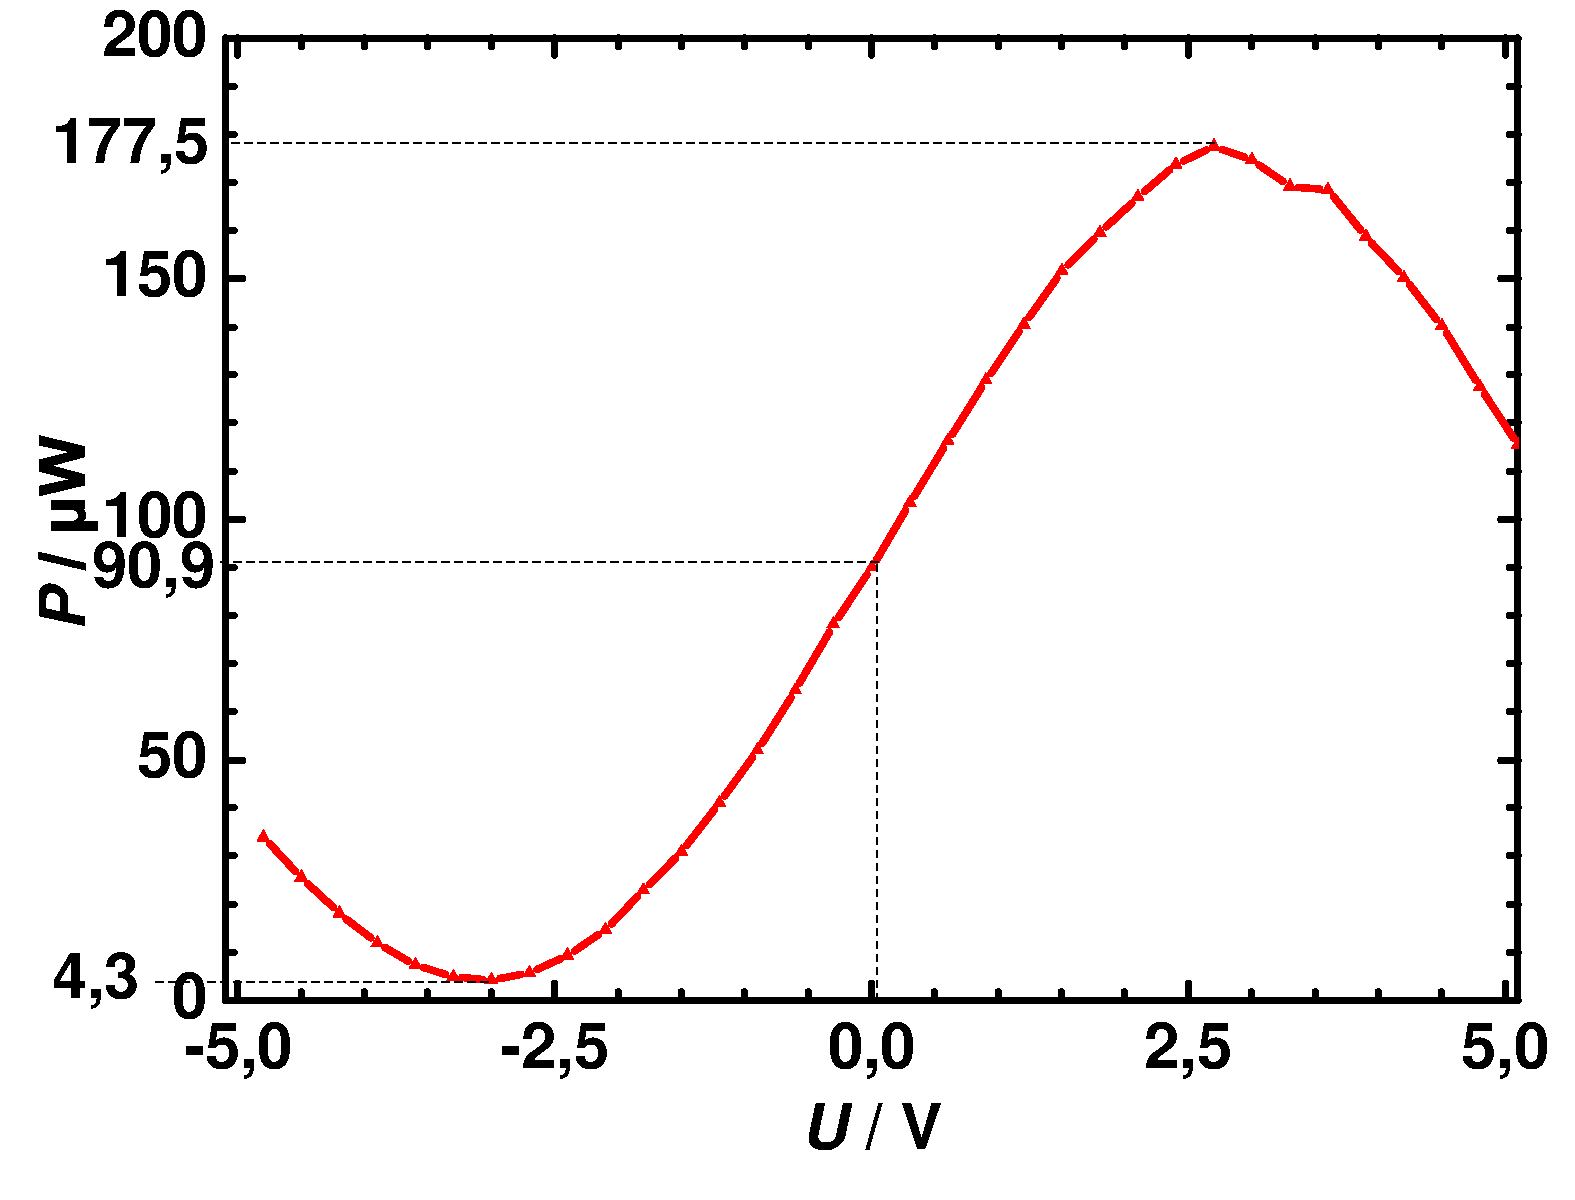
\includegraphics[width=.6\columnwidth]{Grafiken/A_quadratur.pdf}%
\caption{}%
\label{fig:A_quadratur}%
\end{figure}

Figure \ref{fig:A_quadratur} shows the recorded $P$/$U$ curve. It shows a good accordance to the squared sine $P$/$U$ curve of a theoretical MZI modulator.
The maximum optical output power of the MZI is at 2.5~V with 177.5~$\upmu$W. The minimal optical output power is at -3.0~V with 4.3~$\upmu$W. With this the quadrature point can be calculated to be at

\begin{equation}
P\i{out,quadrature}=\frac{177.5~\upmu \mathrm{W}+4.3~\upmu \mathrm{W}}{2}=90.9~\upmu \mathrm{W}\qquad.
\label{eq:}
\end{equation} 
Using a linear approximation in the quadrature point the corresponding voltage can be calculated.

\begin{equation}
\begin{split}
P\i{out}=90~\upmu \mathrm{W} + \frac{103.4~\upmu \mathrm{W}- 78.1~\upmu \mathrm{W}}{0.6~\mathrm{V}}\cdot U\\
U\i{quadrature}=\frac{90.9~\upmu \mathrm{W}-90~\upmu \mathrm{W}}{42.17~\upmu \mathrm{W}/\mathrm{V}}\\
=0.02~\mathrm{V} \quad.
\end{split}
\label{eq:}
\end{equation}
The quadrature point of the transfer function of the modulator was determined to be at $U\i{quadrature}\approx 0~\mathrm{V}$.


\section{Setup B: Optimization of the extinction ratio of the modulator; Q-factor measurement}


\ref{fig:B_setup}\footnote[3]{Luca Alloatti, Materials for the preparation of OKT lab 8}


\begin{figure}%
\centering
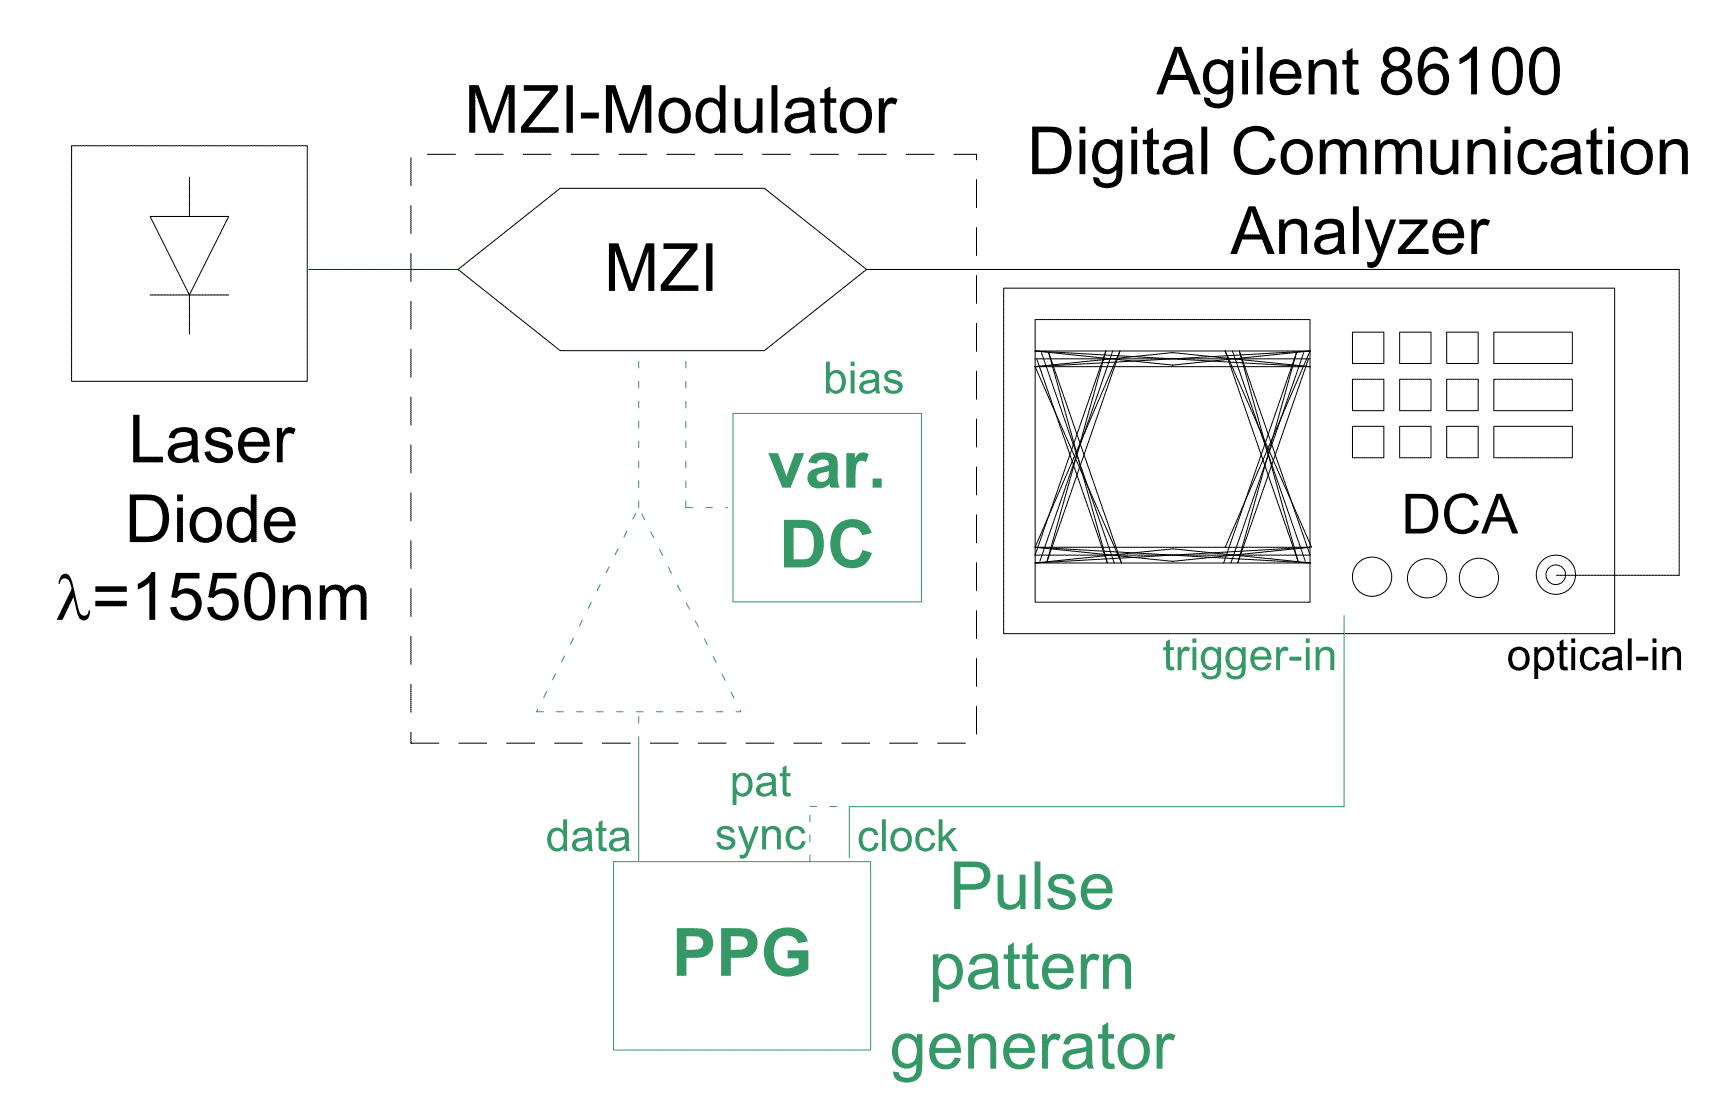
\includegraphics[width=.6\columnwidth]{Grafiken/B_setup.png}%
\caption{Setup B}%
\label{fig:B_setup}%
\end{figure} 